\documentclass[11pt,a4paper]{article}
\usepackage[left=2cm,right=2cm,top=2cm,bottom=2cm]{geometry}
\usepackage{xcolor}
\usepackage{hyperref}
\usepackage{fontawesome5}
\usepackage{titlesec}
\usepackage{graphicx}
\usepackage{enumitem}
\usepackage{caption}
\usepackage{setspace}
\usepackage{tabularx}

% 줄간격 설정
\linespread{1.1}

\hypersetup{
    colorlinks=true,
    linkcolor=blue,
    filecolor=magenta,
    urlcolor=blue,
}

\titleformat{\section}
  {\Large\bfseries}
  {}{0em}
  {}
  [\titlerule]

\titleformat{\subsection}
  {\large\bfseries}
  {}{0em}
  {}

\setlist[itemize]{leftmargin=*, label=--, itemsep=0.3em}

\begin{document}

\begin{minipage}[t]{0.69\textwidth}
{\huge\bfseries Curriculum Vitae}\\[0.8cm]
{\Large\bfseries Dr. Sangdon Park}

\vspace{0.3cm}
Post-Doctoral Researcher\\
Information \& Electronics Research Institute, KAIST\\
KAIST, 291 Daehak-ro, Yuseong-gu, Daejeon 34141, South Korea\vspace{0.3cm}\\
\faEnvelope\ \href{mailto:johnsdpark@gmail.com}{johnsdpark@gmail.com} \hfill \faPhone\ +82-10-2523-3824 \\[0.2cm]
\faGlobe\ \href{https://sangdon-park.github.io/}{sangdon-park.github.io} \hfill \faLinkedin\ \href{https://www.linkedin.com/in/sangdon/}{linkedin.com/in/sangdon}
\end{minipage}%
\hfill
\begin{minipage}[t]{0.3\textwidth}
\vspace{-0.3cm}
\begin{flushright}
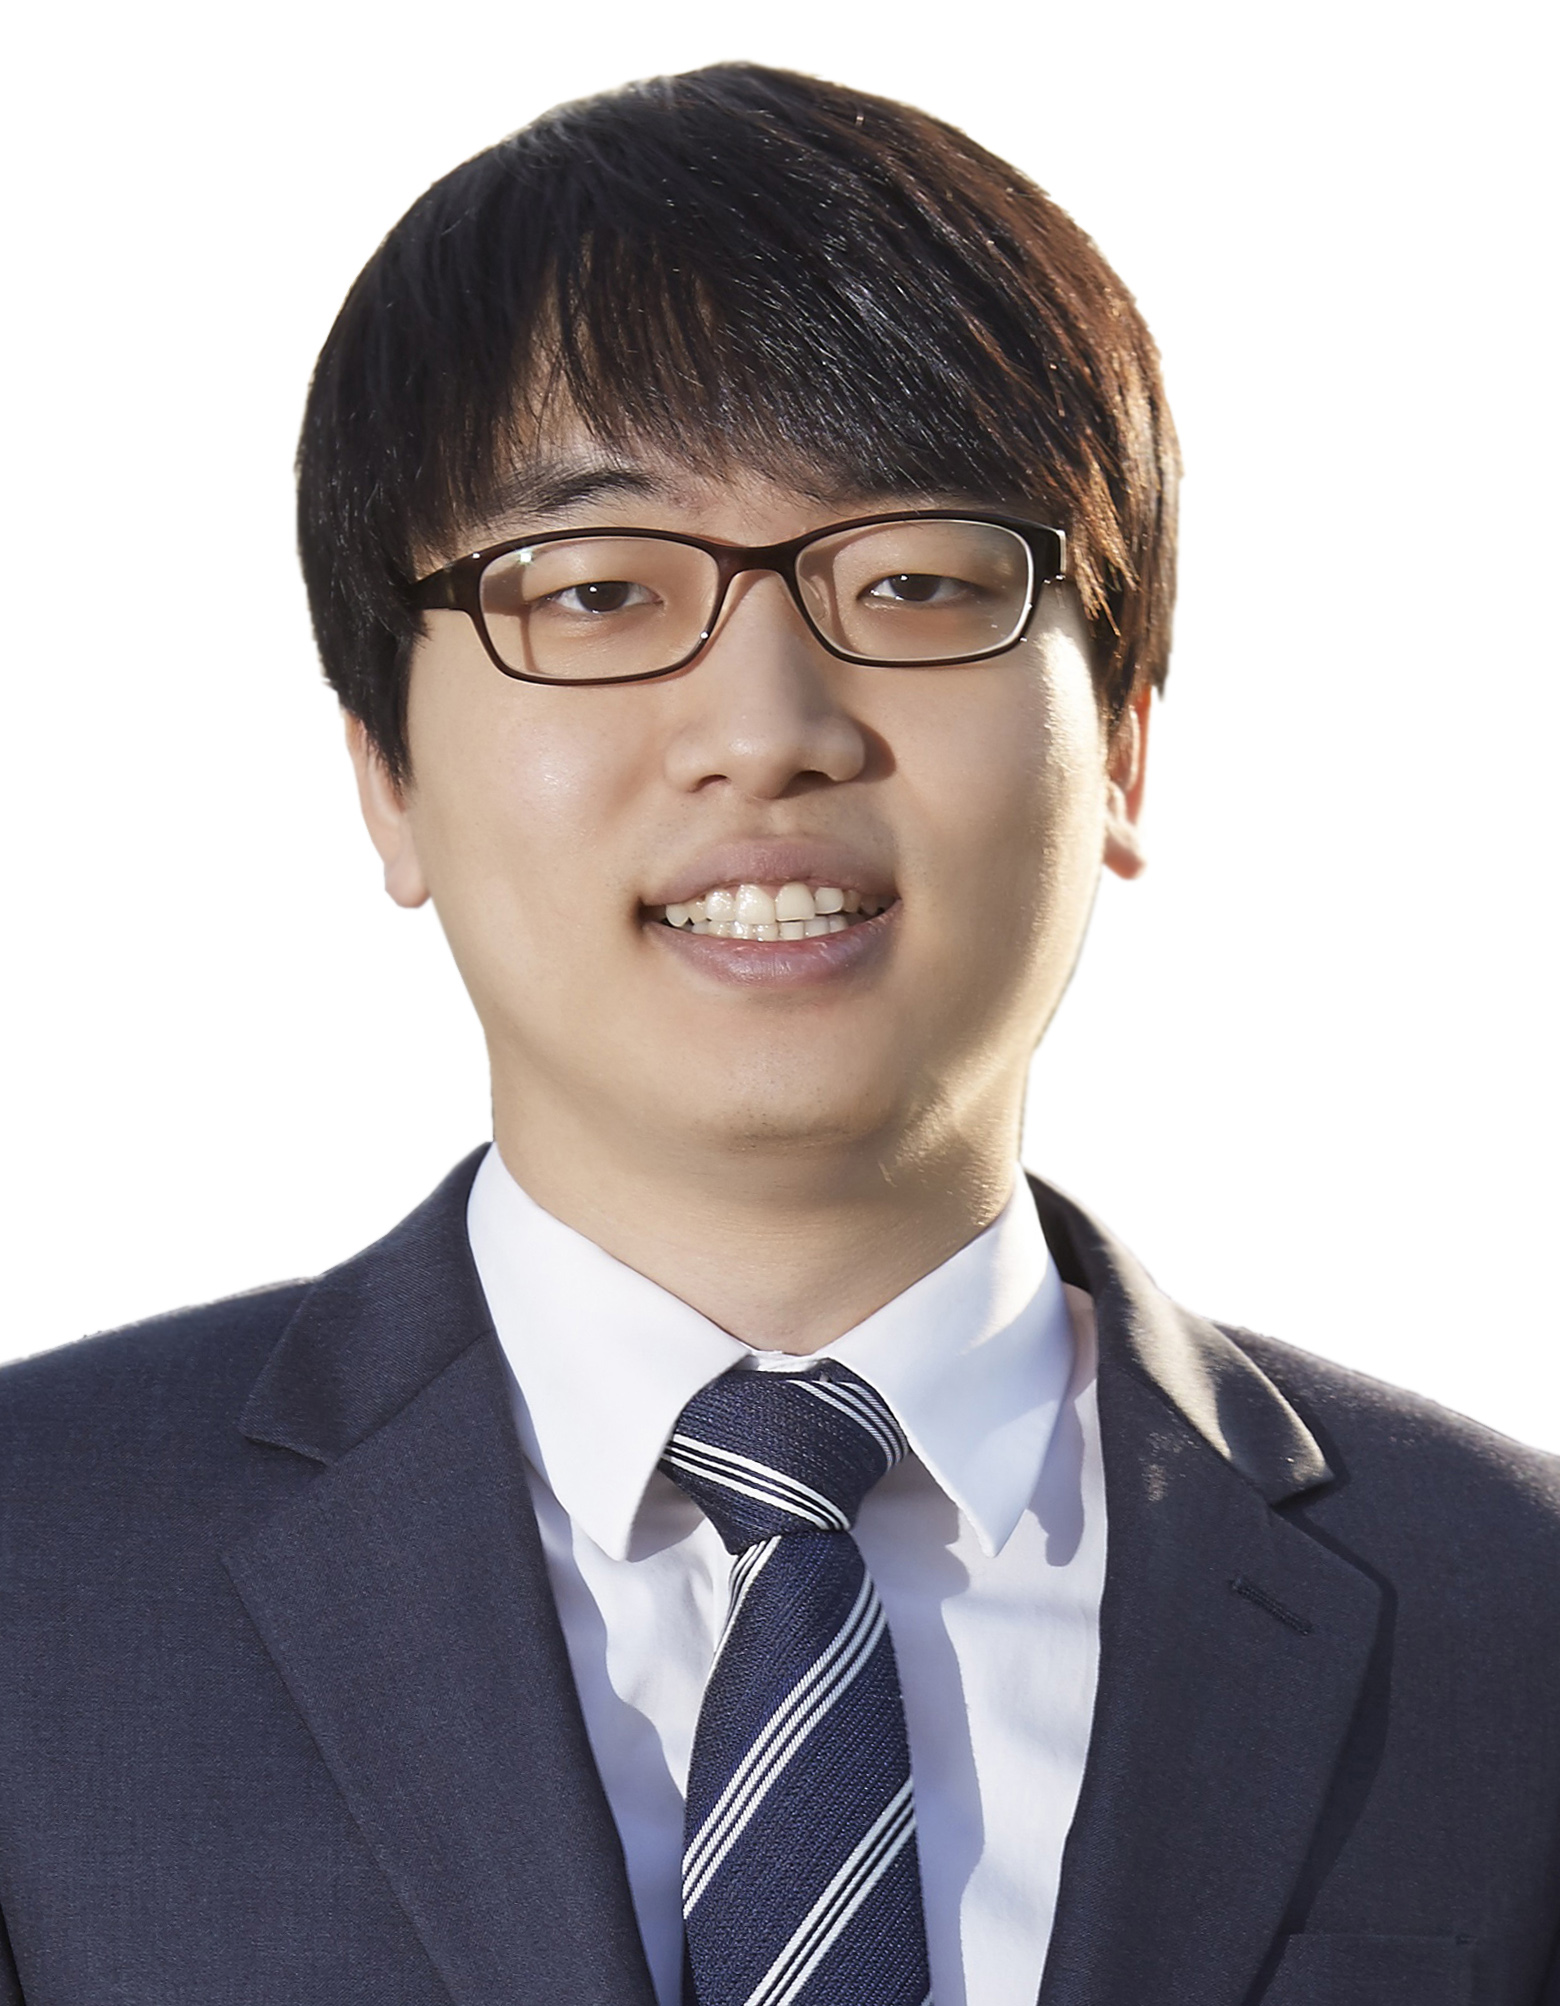
\includegraphics[width=0.7\textwidth]{Sangdon.jpg}
\end{flushright}
\end{minipage}

\vspace{0.3cm}
\linespread{1}
\section{WORK EXPERIENCE}

\subsection*{AI Researcher / Developer (Scheduled), Sayberry Games}
\textit{May 2024 -- Present (Expected)}

\begin{itemize}
    \item Research and development of LLM-based AI characters and interactive game systems
    \item Innovation in game content creation processes using AI technologies
\end{itemize}

\subsection*{Post-Doctoral Researcher, Information \& Electronics Research Institute, KAIST}
\textit{August 2017 -- Present} \hfill \textit{Advisor: Jun Kyun Choi}

\begin{itemize}
    \item Research on edge computing, energy trading, and data market optimization
    \item Exploration and application of AI/LLM technologies
\end{itemize}

\section{PROFESSIONAL SUMMARY}

Dr. Sangdon Park is a distinguished researcher with a strong foundation in wireless networks, smart grids, and edge computing, complemented by a recent and intensive focus on AI and Large Language Model (LLM) applications. He earned his Ph.D. in Electrical Engineering from KAIST in 2017, where his research centered on dynamic energy trading systems within microgrids, leveraging optimization and game theory. Prior to his doctoral studies, he completed his M.S. and B.S. in Mathematical Sciences at KAIST, developing a robust understanding of stochastic processes and queueing theory for wireless communication networks.

Since August 2017, Dr. Park has served as a Post-Doctoral Researcher at the Information \& Electronics Research Institute at KAIST. His work has advanced research in edge computing, energy trading, and data market optimization. A testament to his research excellence is the prestigious \textbf{Sejong Science Fellowship} awarded by the National Research Foundation of Korea in 2022. This fellowship provides substantial funding (approximately \$120,000 per year for up to 5 years) for his role as Principal Investigator in pioneering edge computing research. He also successfully led a significant \textbf{Basic Science Research Program} (NRF Korea, 2018-2022) focused on learning-based energy trading blockchain technology.

In the past year, Dr. Park has directed his focus towards AI/LLM technologies. During this period, he developed an \textbf{Edge Computing GUI Simulator} within one month and an \textbf{AI Character Conversations} project, which demonstrates the creation of natural and complex character interactions for potential applications in game development. This dedicated focus on AI has paved the way for his upcoming role as an AI Researcher/Developer at \textbf{Sayberry Games}, commencing May 2024, where he will drive AI-based interactive experience research. He has also secured an \textbf{AI game development project} valued at 300 million KRW. Dr. Park's current research interests are concentrated on LLM-based system design, AI characters and interactive systems, AI-driven simulation and optimization, and enhancing development productivity through AI tools, continuing to synergize rigorous mathematical modeling with cutting-edge AI methodologies.

\section{EDUCATION}

\begin{tabular}{p{14cm}r}
\textbf{Ph.D. in School of Electrical Engineering, KAIST} & 2013--2017 \\
\\
\textit{Thesis:} Dynamic Energy Trading Scheme for Future Smart Grid & \\
\textit{Advisor:} Prof. Jun Kyun Choi (Media Network Lab.) & \\
\textit{Focus:} Wireless Communications, Smart Grid, Optimization, Game Theory, Energy Big Data & \\
\\
\textbf{M.S. in Department of Mathematical Sciences, KAIST} & 2011--2013 \\
\\
\textit{Thesis:} Throughput Performance Analysis of Optimal Random Access Policies for & \\
Cognitive Radio Networks & \\
\textit{Advisor:} Prof. Ganguk Hwang (Next Generation Communication Networks Lab.) & \\
\textit{Focus:} Stochastic Processes, Queueing Theory, Probability Theory, Wireless Communications & \\
\\
\textbf{B.S. in Department of Mathematical Sciences, KAIST} & 2006--2011 \\
\end{tabular}

\section{GRANTS}

\begin{tabular}{p{14cm}r}
\textbf{Sejong Science Fellowship (Domestic Track), National Research Foundation of Korea} & 2022--Present \\
₩120,000,000 (Korean Won) per year $\approx$ \$100,000 (US Dollars) per year for 3+2 years, Currently in the 4st year of the fellowship & \\
\\
\textbf{Basic Science Research Program, National Research Foundation of Korea} & 2018--2022 \\
₩200,000,000 (Korean Won) $\approx$ \$200,000 (US Dollars) for 4 years & \\
``Learning-based Energy Trading Blockchain Technology using Smart Contract'' & \\
This grant usually supports young professors, and this is a highly exceptional case & \\
\\
\textbf{Brain Korea 21 Plus Program, National Research Foundation of Korea} & 2017--2019 \\
₩45,000,000 (Korean Won) $\approx$ \$45,000 (US Dollars) for 1.5 years & \\
\end{tabular}

\section{PUBLICATIONS}

\subsection{International Journals (* denotes corresponding author, † denotes first author)}
(Total 25 papers: 4 first-authored, 13 corresponding-authored)

\begin{enumerate}[label={[{\arabic*}]}, leftmargin=*, itemsep=0.3em]

% 2024
\item \textbf{Sangdon Park}; Sohee Bae; Joohyung Lee; Youngchul Sung, ``Real-Time Dynamic Pricing for Edge Computing Services: A Market Perspective,'' \textit{IEEE Access}, vol. 12, pp. 134754--134769, 2024.

\item Mohammed, A.; Lee, J.; \textbf{Sangdon Park*}, ``Dynamic Bandwidth Slicing in Passive Optical Networks to Empower Federated Learning,'' \textit{Sensors}, vol. 24, no. 15, 2024.

% 2022
\item Hyeonseok Seo; Hyeontaek Oh; Jun Kyun Choi; \textbf{Sangdon Park*}, ``Differential Pricing-Based Task Offloading for Delay-Sensitive IoT Applications in Mobile Edge Computing System,'' \textit{IEEE Internet of Things Journal}, vol. 9, no. 19, pp. 19116--19131, 2022.

\item Jaeseob Han; Gyeong Ho Lee; \textbf{Sangdon Park*}; Jun Kyun Choi, ``Joint Subcarrier and Transmission Power Allocation in OFDMA-Based WPT System for Mobile-Edge Computing in IoT Environment,'' \textit{IEEE Internet of Things Journal}, vol. 9, no. 16, pp. 15039--15052, 2022.

\item Yue Zang; Yuyang Peng; \textbf{Sangdon Park}; Han Hai; Fawaz Al-Hazemi; Mohammad Meraj Mirza, ``A Novel Cooperative Transmission Scheme in UAV-Assisted Wireless Sensor Networks,'' \textit{Electronics}, vol. 11, no. 4, 2022.

\item Jangkyum Kim; Joohyung Lee; \textbf{Sangdon Park}; Jun Kyun Choi, ``Power Scheduling Scheme for a Charging Facility Considering the Satisfaction of Electric Vehicle Users,'' \textit{IEEE Access}, vol. 10, pp. 25153--25164, 2022.

% 2021
\item Jaeseob Han; Gyeong Ho Lee; \textbf{Sangdon Park*}; Joohyung Lee; Jun Kyun Choi, ``A Multivariate-Time-Series-Prediction-Based Adaptive Data Transmission Period Control Algorithm for IoT Networks,'' \textit{IEEE Internet of Things Journal}, vol. 9, no. 1, pp. 419--436, 2021.

\item Jinhwan Jeon; Yoonjin Hwang; Yongseop Jeong; \textbf{Sangdon Park}; In So Kweon; Seibum B. Choi, ``Lane Detection Aided Online Dead Reckoning for GNSS Denied Environments,'' \textit{Sensors}, vol. 21, no. 20, 2021.

\item Hyeontaek Oh; \textbf{Sangdon Park*}; Jun Kyun Choi; Sungkee Noh, ``Deposit Decision Model for Data Brokers in Distributed Personal Data Markets Using Blockchain,'' \textit{IEEE Access}, vol. 9, pp. 114715--114726, 2021.

% 2020
\item Beomhan Baek; Joohyung Lee; Yuyang Peng; \textbf{Sangdon Park*}, ``Three Dynamic Pricing Schemes for Resource Allocation of Edge Computing for IoT Environment,'' \textit{IEEE Internet of Things Journal}, vol. 7, no. 5, pp. 4292--4303, 2020.

\item Hyeontaek Oh; \textbf{Sangdon Park*}; Gyu Myoung Lee; Jun Kyun Choi; Sungkee Noh, ``Competitive Data Trading Model with Privacy Valuation for Multiple Stakeholders in IoT Data Markets,'' \textit{IEEE Internet of Things Journal}, vol. 7, no. 4, pp. 3623--3639, 2020.

\item Gyohun Jeong; \textbf{Sangdon Park*}; Ganguk Hwang, ``Time Series Forecasting Based Day-Ahead Energy Trading in Microgrids: Mathematical Analysis and Simulation,'' \textit{IEEE Access}, vol. 8, pp. 63885--63900, 2020.

% 2019
\item Jangkyum Kim; Joohyung Lee; \textbf{Sangdon Park}; Jun Kyun Choi, ``Battery-Wear-Model-Based Energy Trading in Electric Vehicles: A Naive Auction Model and a Market Analysis,'' \textit{IEEE Transactions on Industrial Informatics}, vol. 15, no. 7, pp. 4140--4151, 2019.

\item \textbf{Sangdon Park}; Ganguk Hwang; Jun Kyun Choi, ``Optimal Throughput Analysis of Multiple Channel Access in Cognitive Radio Networks,'' \textit{Annals of Operations Research}, vol. 277, no. 2, pp. 345--370, 2019.

\item Yuyang Peng; Jun Li; \textbf{Sangdon Park*}; Konglin Zhu; Mohammad Mehedi Hassan; Ahmed Alsanad, ``Energy-Efficient Cooperative Transmission for Intelligent Transportation Systems,'' \textit{Future Generation Computer Systems}, vol. 94, pp. 634--640, 2019.

\item Jaewon Ahn; Joohyung Lee; \textbf{Sangdon Park}; Hong-Shik Park, ``Power Efficient Clustering Scheme for 5G Mobile Edge Computing Environment,'' \textit{Mobile Networks and Applications}, vol. 24, no. 2, pp. 643--652, 2019.

\item Hyeontaek Oh; \textbf{Sangdon Park*}; Gyu Myoung Lee; Hwanjo Heo; Jun Kyun Choi, ``Personal Data Trading Scheme for Data Brokers in IoT Data Marketplaces,'' \textit{IEEE Access}, vol. 7, pp. 40120--40132, 2019.

\item Sohee Bae; \textbf{Sangdon Park*}, ``Comparison Between Seller and Buyer Pricing Systems for Energy Trading in Microgrids,'' \textit{IEEE Access}, vol. 7, pp. 54084--54096, 2019.

% 2018
\item Nakyoung Kim; \textbf{Sangdon Park*}; Joohyung Lee; Jun Kyun Choi, ``Load Profile Extraction by Mean-Shift Clustering with Sample Pearson Correlation Coefficient Distance,'' \textit{Energies}, vol. 11, no. 9, 2018.

\item Seong-Hwan Kim; \textbf{Sangdon Park*}; Min Chen; Chan-Hyun Youn, ``An Optimal Pricing Scheme for the Energy-Efficient Mobile Edge Computation Offloading with OFDMA,'' \textit{IEEE Communications Letters}, vol. 22, no. 9, pp. 1922--1925, 2018.

\item Busik Jang; \textbf{Sangdon Park*}; Joohyung Lee; Sang-Geun Hahn, ``Three Hierarchical Levels of Big-Data Market Model Over Multiple Data Sources for Internet of Things,'' \textit{IEEE Access}, vol. 6, pp. 31269--31280, 2018.

\item Sanghong Ahn; Joohyung Lee; \textbf{Sangdon Park*}; S.H. Shah Newaz; Jun Kyun Choi, ``Competitive Partial Computation Offloading for Maximizing Energy Efficiency in Mobile Cloud Computing,'' \textit{IEEE Access}, vol. 6, pp. 899--912, 2018.

% 2017
\item \textbf{Sangdon Park}; Joohyung Lee; Ganguk Hwang; Jun Kyun Choi, ``Event-Driven Energy Trading System in Microgrids: Aperiodic Market Model Analysis with a Game Theoretic Approach,'' \textit{IEEE Access}, vol. 5, pp. 26291--26302, 2017.

\item Minkyung Kim; \textbf{Sangdon Park}; Joohyung Lee; Yongjae Joo; Jun Kyun Choi, ``Learning-Based Adaptive Imputation Method with kNN Algorithm for Missing Power Data,'' \textit{Energies}, vol. 10, no. 10, 2017.

% 2016
\item \textbf{Sangdon Park}; Joohyung Lee; Sohee Bae; Ganguk Hwang; Jun Kyun Choi, ``Contribution-Based Energy-Trading Mechanism in Microgrids for Future Smart Grid: A Game Theoretic Approach,'' \textit{IEEE Transactions on Industrial Electronics}, vol. 63, no. 7, pp. 4255--4265, 2016.
\end{enumerate}

\subsection{International Conferences}

\begin{enumerate}[label={[{\arabic*}]}, leftmargin=*, itemsep=0.3em]

% 2021
\item J Lee; M Kim; \textbf{Sangdon Park}; J.K. Choi; Y Hwang, ``Driver Identification for Different Road Shapes Using Vehicle IoT Sensing Data,'' in \textit{Proceedings of the 2021 IEEE International Conference on Consumer Electronics (ICCE)}, Las Vegas, NV, USA, January 10--12, 2021.

% 2018
\item J Han; \textbf{Sangdon Park}; G.H. Lee; M Kim; H Seo; J.K. Choi, ``Energy Trading in Wireless Power Transmission System Considering Nonlinear Rectifier,'' in \textit{Proceedings of the 2018 IEEE 7th Global Conference on Consumer Electronics (GCCE)}, Nara, Japan, October 9--12, 2018.

\item Eunju Yang; Seong Hwan Kim; TaeWoo Kim; Min Su Jeon; \textbf{Sangdon Park}; Chan-Hyun Youn, ``An Adaptive Batch-Orchestration Algorithm for the Heterogeneous GPU Cluster Environment in Distributed Deep Learning System,'' in \textit{Proceedings of the 2018 IEEE International Conference on Big Data and Smart Computing (BigComp)}, Shanghai, China, January 15--17, 2018.

\item Minkyung Kim; \textbf{Sangdon Park}; Kireem Han; Nakyoung Kim; Jun Kyun Choi, ``Dynamics of Electricity Consumers for Classifying Power Consumption Data Using PCA,'' in \textit{Proceedings of the 2018 IEEE International Conference on Big Data and Smart Computing (BigComp)}, Shanghai, China, January 15--17, 2018.

% 2017
\item \textbf{Sangdon Park}; Justin Weimer; Insup Lee, ``Resilient Linear Classification: An Approach to Deal with Attacks on Training Data,'' in \textit{Proceedings of the 8th ACM/IEEE International Conference on Cyber-Physical Systems (ICCPS)}, Pittsburgh, PA, USA, April 18--21, 2017.

% 2016
\item \textbf{Sangdon Park}; Jae Deok Kim; Ganguk Hwang; Jun Kyun Choi, ``Joint Optimal Access and Sensing Policy on Distributed Cognitive Radio Networks with Channel Aggregation,'' in \textit{Proceedings of the 2016 Eighth International Conference on Ubiquitous and Future Networks (ICUFN)}, Vienna, Austria, July 5--8, 2016.

\item Hyeontaek Oh; S.H. Shah Newaz; \textbf{Sangdon Park}; Jun Kyun Choi, ``Maximizing Energy Efficiency in Off-Peak Hours: A Novel Sleep Scheme for WLAN Access Points,'' in \textit{Proceedings of the 2016 IEEE/IFIP Network Operations and Management Symposium (NOMS)}, Istanbul, Turkey, April 25--29, 2016.

\item \textbf{Sangdon Park}; Ganguk Hwang; Jun Kyun Choi, ``Optimal Throughput Analysis of Random Access Policies for Cognitive Radio Networks with Multiple Channel Access,'' in \textit{Proceedings of the 11th International Conference on Queueing Theory and Network Applications (QTNA)}, Wellington, New Zealand, December 13--15, 2016.

% 2013
\item Seonghwa Yun; Kyeongmin Lee; \textbf{Sangdon Park}; Jun Kyun Choi, ``Energy Efficient Relay Selection Scheme with DRX Mechanism in 3GPP LTE Network,'' in \textit{Proceedings of the 2013 International Conference on ICT Convergence (ICTC)}, Jeju Island, South Korea, October 14--16, 2013.
\end{enumerate}

\section{STANDARD ACTIVITIES}

\begin{tabularx}{\textwidth}{X}
\textbf{International Telecommunication Union Telecommunication (ITU-T) Standards} \\[0.2cm]
Representative of South Korea, ITU-T SG13 \& SG5 \hfill \textit{June 2013 -- November 2014}\\
\\[0.3cm]
\textbf{ITU-T SG13 Rapporteurs Meeting} \hfill \textit{June 2013, Geneva, Switzerland}
\\[0.2cm]
\textbf{Sangdon Park}; Seung Hyun Jeon; Jun Kyun Choi; Jeong Yun Kim, ``Consideration of classification of sleep mode control on network equipment,'' SG13RGM-C-06 \\[-0.2cm]
\\
Seung Hyun Jeon; \textbf{Sangdon Park}; Jun Kyun Choi, ``Revised draft Recommendation Y.energyMRM for requesting the consent,'' SG13RGM-C-04 \\[-0.2cm]
\\
Seung Hyun Jeon; \textbf{Sangdon Park}; Jun Kyun Choi; Jeong Yun Kim, ``Consideration of classification for CPU power consumption on network equipment,'' SG13RGM-C-05 \\
\\[0.3cm]
\textbf{ITU-T SG13 Meeting} \hfill \textit{November 2013, Kampala, Uganda} \\[0.2cm]
\textbf{Sangdon Park}; Gyu Myoung Lee; Jun Kyun Choi, ``Proposal of the new draft recommendation Y.energyECN (Energy efficiency class of network equipment),'' COM13-C401-E \\
\\[0.3cm]
\textbf{ITU-T SG13 Rapporteurs Meeting} \hfill \textit{February 2014, Geneva, Switzerland} \\[0.2cm]
\textbf{Sangdon Park}; Jaewon Ahn; Jun Kyun Choi; Gyu Myoung Lee, ``A proposal for definitions of energy efficiency class of network equipment,'' SG13RGM-C-94 \\[-0.2cm]
\\
\textbf{Sangdon Park}; Jaewon Ahn; Jun Kyun Choi; Gyu Myoung Lee, ``Revised texts for a main chapter of draft recommendation,'' SG13RGM-C-75 \\[-0.2cm]
\\
\textbf{Sangdon Park}; Jun Kyun Choi; Gyu Myoung Lee, ``A proposal for definitions of energy efficiency class of network equipment,'' SG13RGM-C-75 \\
\end{tabularx}

\section{TEACHING ACTIVITIES}

\begin{tabular}{p{14cm}r}
\textbf{Design Assistant} & Spring 2014 \\
``Introduction to Electronics Design Lab.'', School of Electrical Engineering at KAIST & \\
\\
\textbf{Counseling Assistant} & Fall 2013 \\
School of Electrical Engineering at KAIST & \\
\\
\textbf{Teaching Assistant} & Fall 2012 \\
Calculus II, Department of Mathematical Sciences at KAIST & \\
\\
\textbf{Teaching Assistant} & Spring 2012 \\
Calculus I, Department of Mathematical Sciences at KAIST & \\
\\
\textbf{Teaching Assistant} & Fall 2011 \\
Introduction to Linear Algebra, Department of Mathematical Sciences at KAIST & \\
Probability and Statistics, Department of Mathematical Sciences at KAIST & \\
\end{tabular}

\end{document}
